\chapter{Deseño e implementación}
\minitoc
% \label{chap:Desenoeimplementacion}
% \vspace{0.5cm}

%%%%%%%%%%%%%%%%%%%%%%%%%%%%%%%%%%%%%%%%%%%%%%%%%%%%%%%%%%%%%%%%%%%%%%%%%%%%%%%%
% Objetivo:                        %
%%%%%%%%%%%%%%%%%%%%%%%%%%%%%%%%%%%%%%%%%%%%%%%%%%%%%%%%%%%%%%%%%%%%%%%%%%%%%%%%

  \lettrine{E}{n} este capítulo veremos os detalles de deseño e implementación 
de diversas partes do proxecto así como falaremos das decisións tomadas con 
respecto a utilización das tecnoloxías.

  \section{ReactJS e Flux}
    \subsection{Introdución e elección da tecnoloxía}
    Actualmente o mundo das aplicacións móbiles está en pleno crecemento e cada 
vez é máis facil atopar como incluso pequenos comercios ou incluso eventos 
teñen a súa propia aplicación móbil.

    A sociedade está a cambiar un soporte tradicional como é o papel en todas 
os aspectos da vida, dende a publicidade ata a propia xestión e todo estase a 
dixitalizar, facilitando o traballo humano e reducindo os custes a medio prazo.

    Neste contexto decidíuse optar por realizar unha aplicación móbil 
híbrida, con tecnoloxías web, xa que se pode observar un movemento nos últimos 
anos cara este tipo de tecnoloxías que permiten desenvolver únicamente unha 
aplicación e executala nos diversos sistemas operativos móbiles existentes sen 
ter que desenvolver unha aplicación concreta para cada un de eles.

    Tras unha análise das diversas linguaxes e frameworks que podían 
ser utilizados para este fin, finalmente optouse por utilizar ReactJS pola sua 
flexibilidade fronte a outras alternativas como AngularJS ou EmberJS.

    Estas alternativas centranse en ofrecer un framework moi completo buscando 
cubrir todas as tecnoloxías dentro de unha aplicación como o enrutado de urls, 
a internacionalización ou os servizos fronte a React que únicamente trata de 
cubrir a xestión das vistas e do seu estado, dando total liberdade para 
escoller a tecnoloxía que se precise para o resto de compoñentes dunha 
aplicación.

    Así mesmo tamén cómpre destacar a existencia de React Native, unha 
tecnoloxía baseada en React que permite crear aplicacións móbiles con 
tecnoloxías web e con unha experiencia de usuario exactamente igual a unha 
aplicación nativa tradicional.

    Unha vez selecciado React, optamos por seguir a arquitectura máis habitual 
dentro de este tipo de aplicacións, Flux, a través da librería Reflux.

    \subsection{Elementos básicos}
      \subsubsection{Compoñentes de React}
      React é unha librería de Javascript que nos permite xestionar de xeito 
sinxelo as vistas da nosa aplicación a través de diversos elementos denominados 
compoñentes.

      React permítenos escribir os nosos compoñentes con unha sintaxis moi 
similiar a HTML pero posteriormente traduce esta sintaixs a código javascript 
habitual polo que podemos decir que estamos escribindo páxinas web únicamente 
con funcións de javascript.

      A idea principal é reutilizar e agrupar compoñentes para formar o que 
tradicionalmente chamamos vistas e que a súa vez poden ter un estado.
      Este estado pode variar modificando as vistas, como por exemplo, 
engádese un novo gol na lista de eventos e React encárgase de volver a 
renderizar únicamente a parte da vista que cambiou, polo que é tremendamente 
eficiente.

      \subsubsection{Arquitectura Flux}
      Flux é unha arquitectura que básicamente propón o seguinte esquema:

        \begin{figure}[h!]
          \begin{center}
          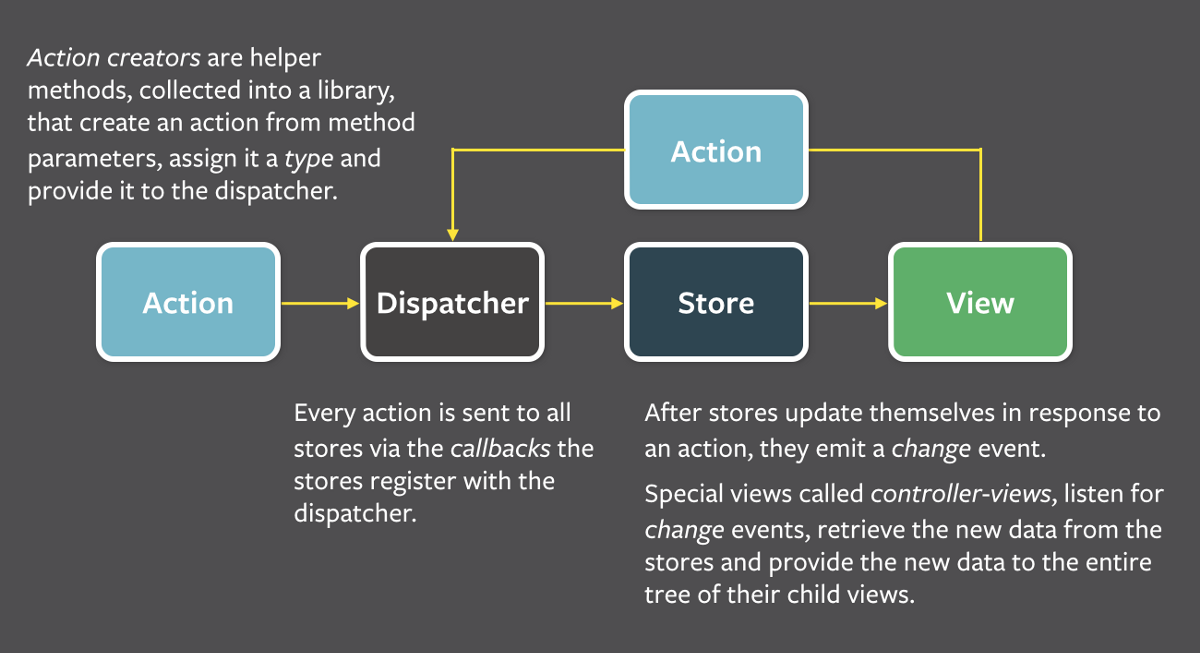
\includegraphics[width=\textwidth]{./img/flux.png}
          \caption{Esquema da arquitectura Flux}
          \end{center}
        \end{figure}

        \paragraph{Actions}
        A vista atópase formada por unha serie de compoñentes de React que son 
capaces de disparar as Actions, que funcionan de xeito similar a eventos, por 
exemplo ao pulsar un botón e que avisán ao Dispatcher.
        \paragraph{Dispatcher}
        O Dispatcher é o encargado de recibir e enrutar as Actions disparadas 
cara as Stores.
        \paragraph{Stores}
        Estas Stores son as encargadas de xestionar o estado dos compoñentes e 
toda a lóxica necesaria para actualizar o estado co novo cambio.

        Se por exemplo ao pulsar un botón debería cambiar un texto que esa no 
compoñente, poderíamos ter este texto almacenado no estado dentro dunha Store e 
inicializado a un valor baleiro.
        Unha vez se fai click no botón, unha Action chamará a unha Store que é 
a que contén a información sobre cómo cambiar o texto do estado e React 
encargarase de volver a pintar o novo valor do estado, dentro do seu compoñente.

      \subsubsection{Implementación de Flux. Reflux.}
      Flux é unha arquitectura, unha especie de patrón de desenvolvemento pero 
existen diversas implementacións da mesma e neste proxecto decidímonos por 
utilizar Reflux.

      O funcionamento é moi similar pero con algúns matices, por exemplo ao non 
existir un único Dispatcher central que enruta as Actions se non que todas as 
Stores están escoitando e reaccionan cando teñen un método para responder a 
Action.

     Vexamos un exemplo práctico:

     \begin{lstlisting}[frame=single]
      let TextActions = Reflux.createActions([
        "updateText"
      ])
    \end{lstlisting}

    Definiríamos unha Action que queremos lanzar e crearíamos unha Store que 
escoite as TextActions e que implemente unha función onUpdateText que será a 
que reciba o novo valor e actualizará o estado.

     \begin{lstlisting}[frame=single]
        let TextStore = Reflux.createStore({
          listenables: TextActions,
          init: function () {
            this.state = ''
          },
          getInitialState: function () {
            return this.state
          },
          onUpdateText: function (newText) {
            this.state = newText
            this.trigger(this.state)
          }
        })
    \end{lstlisting}

    Por último definir o compoñente. Deberá incluir unha lista de mixins onde 
indicarlle qué Stores reaccionan ante eventos que se lancen dende este 
compoñente, neste caso, a TextStore.

    O compoñente tamén terá un método render no que definir o que poderíamos 
chamar informalmente o ``modelo'' do que queremos renderizar e que inclúe un 
enlace para cambiar o texto mostrado.

    Dito enlace reacciona cando se fai click e chama ao método 
handleChangeTextClick que lanza a Action para que a Store a intercepte, cambie 
o estado e React renderice de novo, únicamente o que cambiou.



     \begin{lstlisting}[frame=single]
      let EndReport = React.createClass({
        mixins: [
          Reflux.connect(TextStore, 'text')
        ],
        handleChangeTextClick: function () {
          TextActions.updateText('Nuevo texto a renderizar')
        }
      render: function () {
          return (
            <p>{this.state}</p>
            <a onClick={this.handleChangeTextClick}>Change text</a>
          )
        }
      })
    \end{lstlisting}


    \subsection{Estructura da aplicación}
    
    \paragraph{App}

      \begin{description}
        \item [Tests] Carpeta onde se poden atopar os tests da aplicación. De 
momento só se dispón de tests da capa de servizos.
        \item [i18n] Nesta localización pódese atopar a internacionalización, 
coas cadeas dentro da subcarpeta de ``messages`` e coa descrición das mesmas 
para cada compoñente de React dentro de ''descriptors`` coa idea de darlle 
contexto e facilitarlle ao traductor a súa labor.
        \item [Cordova app] Aquí podemos atopar a configuración para compilar a 
aplicación aos diversos dispositivios móbiles.
        \item [Src/app] Estructura principal da aplicación
        \begin{description}
          \item [Actions] Lista de ficheiros de accións a disparar agrupados 
cada un pola store que os implementa.
          \item [API] Contén a configuración, as urls da aplicación e a 
factoría utilizada para a inxección de dependencias dos servizos que 
explicaremos máis adiante.
          \item [Components] Lugar onde se poden atopar todos os compoñentes 
que forman as vistas da aplicación. 
          \item [Daos] Entidades que abstraen dos servicios a definición do 
acceso a base de datos, facilitando que sexa sinxelo cambiar dita base de datos 
se é preciso.
          \item [Models] Contén a definición dos modelos da aplicación, tanto as 
entidades que se almacenan en base de datos como de cercas clases que son 
utilizadas pola aplicación como as que definen os deportes ou a implementación 
dos tipos de eventos.
          \item [Services] Estas clases conteñen a lóxica de negocio da 
aplicación.
          \item [Stores] Lista de ficheiros que conteñen e xestionan o estado da 
aplicación diferenciando a lóxica de negocio, que se almacena nos servizos, da 
xestión do estado dos compoñentes de React.
          \item [app.js] Ficheiro de inicialización da aplicación que se encarga 
de arrancar o enrutador e executa a aplicación ben en modo web ou ben en modo 
aplicación móbil en función da configuración definida.
          \item [router.jsx] É o encargado de poñer en relación as urls da 
aplicación cos compoñentes que corresponden a cada unha e donde se introduce 
tamén a información sobre a internacionalización.

        \end{description}

      \end{description}


  \section{Bases de datos e funcionamento offline}
  O mundo das bases de datos está a cambiar enormemente nos últimos anos coa 
aparición das bases de datos non relacionáis, neste caso concreto, era preciso 
dispoñer de unha base de datos no cliente que permitise almacenar os 
datos das actas dos encontros de forma offline xa que o árbitro do encontro 
pode non ter cobertura e debería poder cubrir a súa acta da mesma forma.

  Ante este requisito cabe pensar nas bases de datos lixeiras como SQLite que 
se utilizan habitualmente nas aplicacións móbiles pero ditas bases de datos non 
poden ser executadas directamente nun navegador web, polo que finalmente se 
optóu por utilizar PouchDB, unha base de datos orientada a documentos e creada 
sobre o LocalStorage do navegador, pensada dende o primeiro momento para 
crear aplicacións web que funcionen de forma desconectada.

    \subsection{PouchDB}
    As actas electrónicas son documentos que unha vez sexan creadas, apenas 
serán modificadas e neste tipo de datos son as bases de datos orientadas a 
documentos as que mellor funcionan.

    A elección de PouchDB foi sobre todo motivada polas súas características de 
ser lixeira, multinavegador e sobre todo, facilitar a sincronización contra 
unha base de datos remota, neste caso, CouchDB.

    \subsection{CouchDB}
    CouchDB é a base de datos non relacional que se utiliza como base de datos 
central en remoto coa cal sincronizará a PouchDB que se atopa na aplicación que 
utilizará o árbitro.

    Esta base de datos é tremendamente versatil e sinxela de utilizar xa que 
implementa unha API REST e a forma de interactuar con ela basease simplemente 
en enviar documentos JSON a través de sinxelas peticións HTTP cara a súa API.

    Destaca pola súa extensa comunidade e por ser altamente dispoñible e 
tolerante a erros pero eventualmente inconsistente pero sobre todo pola súa 
xestión de conflictos que comentamos a continuación.

    \subsection{Sincronización e xestión de conflictos}
    Probablemente o maior reto a hora de enfrentarse a unha aplicación con 
funcionamento offline é a xestión de conflictos entre os datos.

    En este caso en concreto, existe a problemática de que por múltiples 
motivos, un acta sexa modificada en dous lugares ao mesmo tempo, tanto polo 
árbitro no seu teléfono como pola persoa encargada da xestión da federación 
polo que resulta imprescindible non perder información e ser capaces de 
mostrarlle a totalidade da información ao xestor da federación para que este 
poida seleccionar cales datos son os reais.

    Neste punto é donde CouchDB resulta moi útil xa que a propia base de datos 
se encarga de almacenar un árbol co histórico de revisións que se producen 
sobre un documento e así se poderían mostrar ao usuario para que seleccione a 
correcta en caso de conflicto.

  \section{App híbrida con Apache Cordova}
  O obxectivo do proxecto é poder utilizalo en múltiples dispositivos móbiles 
co fin de facilitar que calquera árbitro poida utilizala independentemente do 
sistema operativo que teña o seu teléfono ou tableta.

  É por isto que é fundamental a utilización dun sistema que permita este 
desenvolvemento multiplataforma como é o caso de Apache Cordova que facilita o 
acceso aos elementos do dispositivo como sensores, datos, estado de rede... a 
través dunha serie de APIs estandar.

  Actualmente non se está a utilizar ningunha de estas funcionalidades pero si 
é posible que nun futuro cercano se decidan implementar novas características 
que si precise o acceso a este tipo de elementos como pode ser por exemplo o 
micrófono para que o árbitro poida gardar as incidencias dun partido como notas 
de voz en lugar de escribilas.

  A continuación podemos ver un esquema sobre a arquitectura dunha aplicación 
sobre Apache Córdova:

    \begin{figure}[h!]
      \begin{center}
      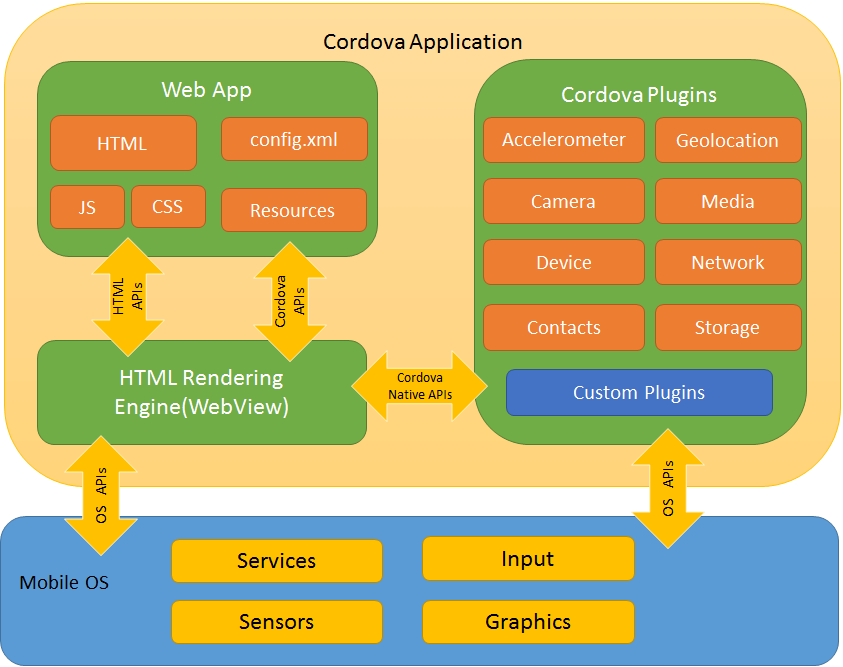
\includegraphics[width=0.8\textwidth]{./img/cordova_arquitectura.png}
      \caption{Arquitectura de unha aplicación con Apache Cordova}
      \end{center}
    \end{figure}

  Básicamente a aplicación executase como unha aplicación web normal sobre un 
WebView, un motor de renderizado de HTML que pode interactuar coas APIs nativas 
do dispositivo a través dunha serie de plugins que Cordova provee.

  Para executar a aplicación únicamente é preciso crear un proxecto de Cordova, 
engadir os ficheiros da aplicación, as plataformas para as que se desexe xerar 
o proxecto e construilo.

  \section{Interface gráfica e usabilidade}
  A importancia da interface gráfica en este proxecto é crucial, debido a que a 
aplicación será utilizada por persoas de un amplísimo rango de idades, a 
usabilidade é o valor máis importante.

  A nivel de deseño a aplicación separase en catro grandes bloques:

  \begin{figure}[h!]
    \begin{center}
    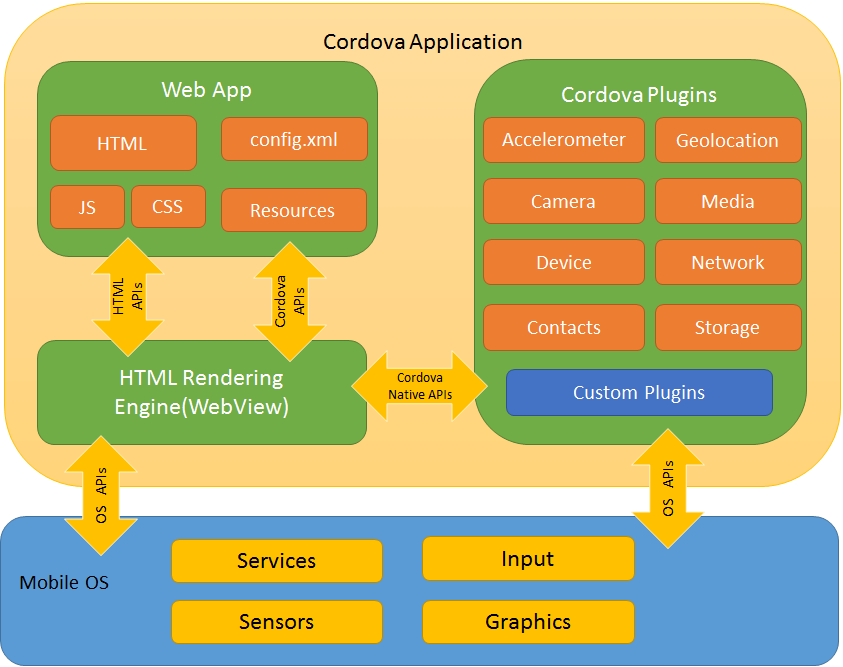
\includegraphics[width=0.2\textwidth]{./img/cordova_arquitectura.png}
    \caption{Estructura da aplicación gráficamente.}
    \end{center}
  \end{figure}

    \subsection{Elementos comúns}
    Para facilitar o desenvolvemento da aplicación creáronse varios 
compoñentes de React xenéricos que permiten realizar tarefas comúns a múliples 
partes da aplicación e polo tanto que son utilizados dende outros compoñentes 
de React.

      \subsubsection{Menú lateral esquerdo}
      É o menú principal da aplicación e que se mostra ao pulsar no botón 
superior esquerdo da aplicación dende a maior parte de vistas da aplicación.

      Este menú desplegable mostra actualmente o logotipo de VACmatch e unha 
serie de enlaces entre os que se atopan as páxinas de configuración e de 
''acerca de``.

      Para xestionar os enlaces que se mostran en cada páxina de forma 
internacionalizada e para permitir dispoñer dos elementos nun sitio 
centralizado creouse o compoñente ''LeftMenuItems''.
      Este compoñente contén varias listas con items para introducir dentro do 
menú lateral esquerdo e que se poden editar ou engadir outras se é 
preciso.

      Utilizase tamén a ``MenuStore'' para xestionar os elementos que se atopan 
en cada momento no menú e pódese utilizar a Action ``setLeftMenu'' para 
modificar os elementos que o compoñen en calquera momento, por exemplo, ao 
entrar en unha nova vista.

      \begin{figure}[h!]
        \begin{center}
        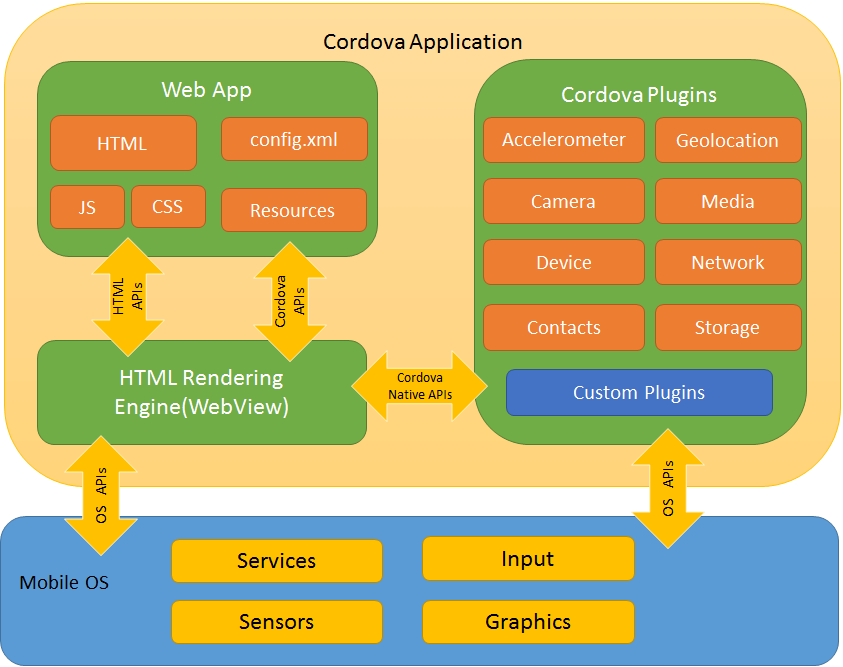
\includegraphics[width=0.2\textwidth]{./img/cordova_arquitectura.png}
        \caption{Menú lateral esquerdo.}
        \end{center}
      \end{figure}

      \subsubsection{Enlaces do menu superior dereito}
      O funcionamento de este menú é moi similar ao anterior só que este 
non dispón de compoñente propio e únicamente é preciso chamar a Action 
``setRightMenu'' para colocar a listaxe cos novos elementos a mostrar no menú 
desplegable.

      A función debe recibir unha lista de obxectos que deben contar cos 
seguintes atributos:

      \begin{description}
       \item [text] Texto a mostrar polo item.
       \item [url] Url a donde ir ao facer click no botón.
       \item [callback] Función de callback a executar unha vez se 
redirixa a aplicación a url indicada (Opcional).
      \end{description}

      \begin{figure}[h!]
        \begin{center}
        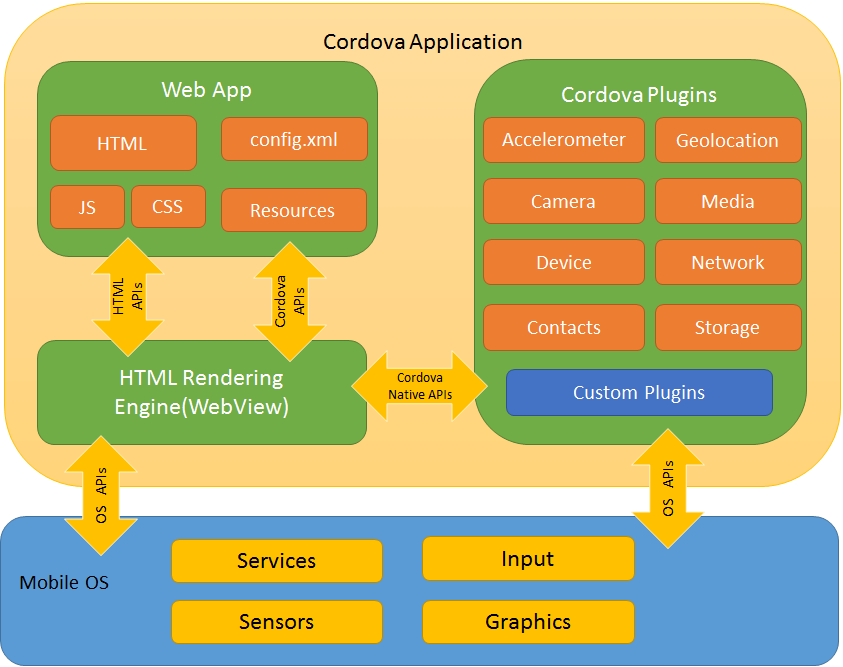
\includegraphics[width=0.2\textwidth]{./img/cordova_arquitectura.png}
        \caption{Menú desplegable dereito.}
        \end{center}
      \end{figure}


      \subsubsection{Información e axustes}
      Toda aplicación debe conter un apartado de información sobre a mesma, e 
en este caso móstrase ademáis as diversas redes sociais do proxecto e o 
repositorio de código en GitHub para que calquera poida contribuir ao proxecto.

      Por outro lado tamén se ten en conta que toda aplicación debe ser 
personalizable en certa medida, de momento non se dispón de opcións máis ca 
cambiar de idioma pero cando exista a necesidade de incorporar 
novos elementos de configuración, este será o apartado onde os usuarios poderán 
modificar ditas opcións.

      \begin{figure}[h!]
        \begin{center}
        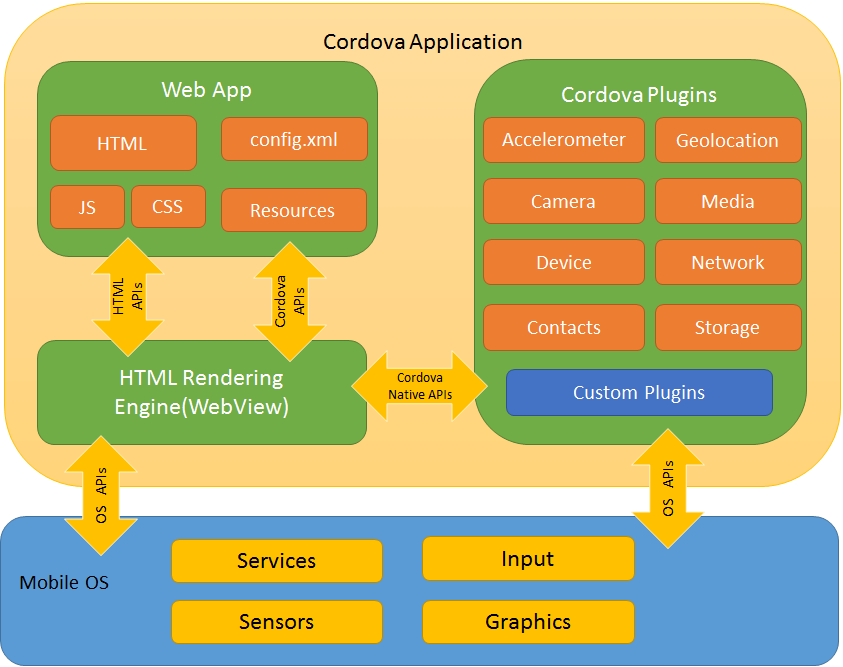
\includegraphics[width=0.2\textwidth]{./img/cordova_arquitectura.png}
        \caption{Ventanas de información e axustes.}
        \end{center}
      \end{figure}

      \subsubsection{SnackBar}
      Inicialmente xurdíu a necesidade de comunicarlle ao usuario os erros que 
se producen na aplicación, casos concretos como introducir un usuario 
incorrecto ou tratar de eliminar un evento de comezo de partido antes de 
eliminar o de fin do mesmo, deben mostrar un aviso ao usuario.

      É por iso que se decidíu crear unha ``SnackBar'', unha pequena barra que 
xurde a modo de aviso na parte inferior da pantalla durante uns segundos para 
mostrar información.

      Inicialmente pensouse para mostrar os erros pero tamén resulta de 
utilidade a hora de mostrarlle outra información ao usuario como cando un 
evento é engadido correctamente.

      \begin{figure}[h!]
        \begin{center}
        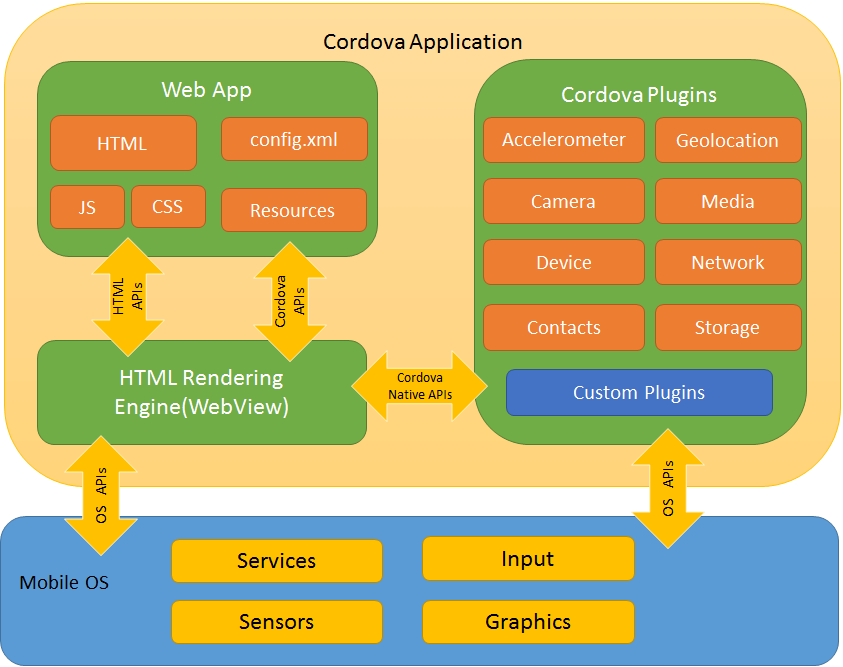
\includegraphics[width=0.2\textwidth]{./img/cordova_arquitectura.png}
        \caption{SnackBar para informar ao usuario.}
        \end{center}
      \end{figure}

      \subsubsection{Autenticación}
      A autenticación é fundamental en esta aplicación xa que únicamente os 
usuarios con acceso poden crear ou modificar actas, neste contexto foi preciso 
crear un compoñente de autenticación que se encargue de realizar esta tarefa de 
comprobar se o usuario iniciou sesión na aplicación, sempre que se carguen os 
compoñentes.

      Unha clase sinxela que deben extender aqueles compoñentes que so poidan 
ser accedidos se o usuario está autenticado, o ``AuthenticatedComponent'' e que 
redirixe a aplicación a páxina de iniciar sesión en caso de non poder atopar un 
usuario na sesión.

    \begin{lstlisting}[frame=single, caption=Compoñente de autenticación.]
export default (ComposedComponent) => {
  let AuthenticatedComponent = React.createClass({
    mixins: [
      Reflux.connect(AuthStore, 'auth'),
      History
    ],

    componentWillMount: function (transition) {
      if (config._env !== 'development') {
      // This method is called before transitioning to this component.
      // If the user is not logged in, we’ll send him or her to the Login page.
        if (!AuthStore.isLoggedIn()) {
          this.history.pushState(null, urls.login.show)
        }
      }
    },

    render: function () {
      return (
        <ComposedComponent
        {...this.props} />
      )
    }
  })
  return AuthenticatedComponent
}
    \end{lstlisting}

    Ao mesmo tempo, este compoñente permítenos aportar unha funcionalidade 
diferente en caso de atoparnos en modo ``desenvolvemento'', saltando a 
comprobación de se o usuario ten sesión iniciada e permitíndonos acceder a 
calquera páxina sen ter que iniciar sesión cada vez que se recarga a páxina.

      \subsubsection{Lista de tabs}
      \todo{Revisar titulo e definición de lapelas}
      Durante o desenvolvemento percatámonos de que é habitual a necesidade de 
utilizar unha lista de elementos divididos en varias lapelas, tanto á hora de 
mostrar a lista de xogadores dos equipos como a hora de asinar un acta ou 
engadir novos eventos.

      É por isto que se creou un compoñente xenérico que permite incorporar 
unha lista de lapelas e unha lista de elementos para cada unha de elas, 
xenerando de xeito sinxelo e xenérico estas vistas xa que é posible 
pasarlle calquera tipo de elemento de tipo Item a esta lista.

    \subsection{Iniciar sesión}
    Aquí podemos atopar a páxina inicial da aplicación que mostra a 
posibilidade de que un usuario da aplicación poidan iniciar sesión cos seus 
datos de acceso así como, pulsando o botón de rexistro, pode crearse un novos 
usuario dentro da aplicación que lle permita crear actas de xeito manual.

    Entre os múltiples parámetros que o usuario pode cubrir atópase un código 
PIN que lle permitirá asinar as actas dos encontros que arbitre.

    Cómpre mencionar que, aparte das páxinas de configuración da aplicación e 
de ``acerca de'', esta é a única vista accesible para usuarios sen autenticar e 
calquera intento de acceso a algunha de esas páxinas redirecionará ao usuario a 
esta páxina de inicio de sesión.

      \begin{figure}[h!]
        \begin{center}
        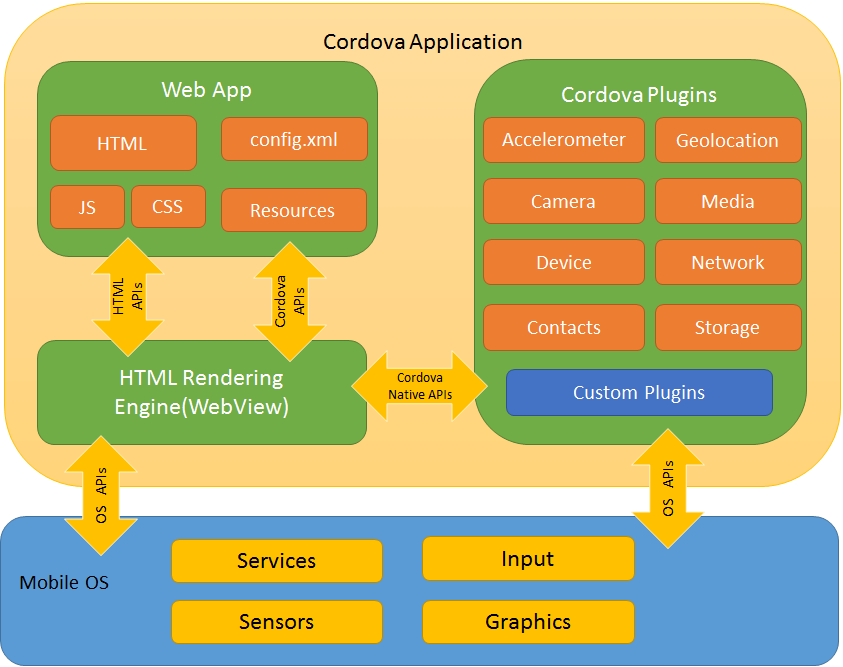
\includegraphics[width=0.2\textwidth]{./img/cordova_arquitectura.png}
        \caption{Vista de inicio de sesión.}
        \end{center}
      \end{figure}

    \subsection{Listado de actas}
    En esta sección poderemos ver a lista de actas que un árbitro ten 
asignadas, divididas en dúas lapelas, por un lado as de próximos partidos a 
arbitrar e por outro aquelas nas que o encontro xa rematóu e que non é habitual 
que sexan accedidas.

    Cada un dos elementos que se mostra permítenos modificar a información 
básica da acta, tanto o nome dos equipos como o lugar de celebración ou a data 
por se é preciso e incluso se podería eliminar a acta e todos os elementos 
que a compoñen se é preciso.

    Ademáis, esta páxina danos a opción de engadir unha nova acta se é preciso, 
un caso fundamental xa que por múltiples razóns poderíase dar o caso de que a 
aplicación de un árbitro non sincronice as súas actas coas existentes na base 
de datos da federación, polo que o árbitro debe poder crear un acta baleira de 
xeito manual incluso sen ter conexión a internet.

      \begin{figure}[h!]
        \begin{center}
        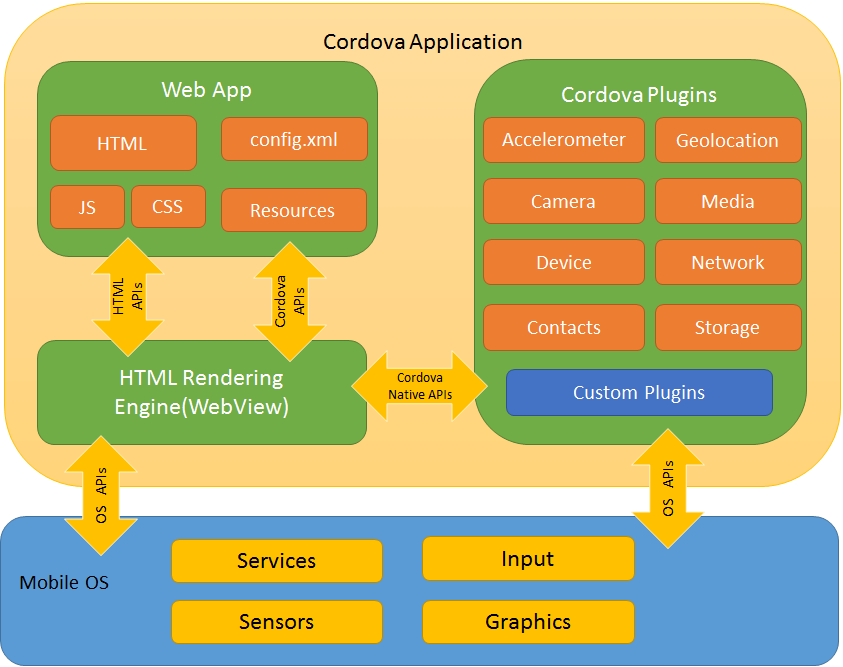
\includegraphics[width=0.2\textwidth]{./img/cordova_arquitectura.png}
        \caption{Listado de actas.}
        \end{center}
      \end{figure}

    \subsection{Acta}
    Esta é a parte central da aplicación, con total seguridade será o lugar 
onde os usuarios pasarán a gran maioría do seu tempo de uso da aplicación xa 
que é o punto central do desenvolvemento dun partido.

    A acta dun encontro deportivo é un elemento con gran cantidade de 
información e que pode ser visualizada sen apenas esforzo xa que se atopa 
toda representada únicamente en unha folla de papel.

    É por iso que dende o primeiro momento se tiña claro que había que tratar 
de manter esa sinxeleza de uso pero, evidentemente, era imposible acceder a 
toda esa información en unha sola vista dentro de un soporte de un tamaño tan 
pequeno como é un teléfono móbil.

    Entón o enfoque foi un pouco diferente e tratouse de facer que o proceso de 
cubrir un acta resultase o máis interactivo posible, mostrando na pantalla 
central únicamente a información indispensable para o árbitro que está a 
cubrila.

    Finalmente móstranse os nomes dos equipos que están a competir con un 
enlace para ver os seus xogadores, dóus campos de resultados, un 
cronómetro, un botón de edición, un botón para mostrar os eventos que 
ocorreron e os diversos eventos que poden ser utilizados para este encontro.

    \begin{figure}[h!]
      \begin{center}
      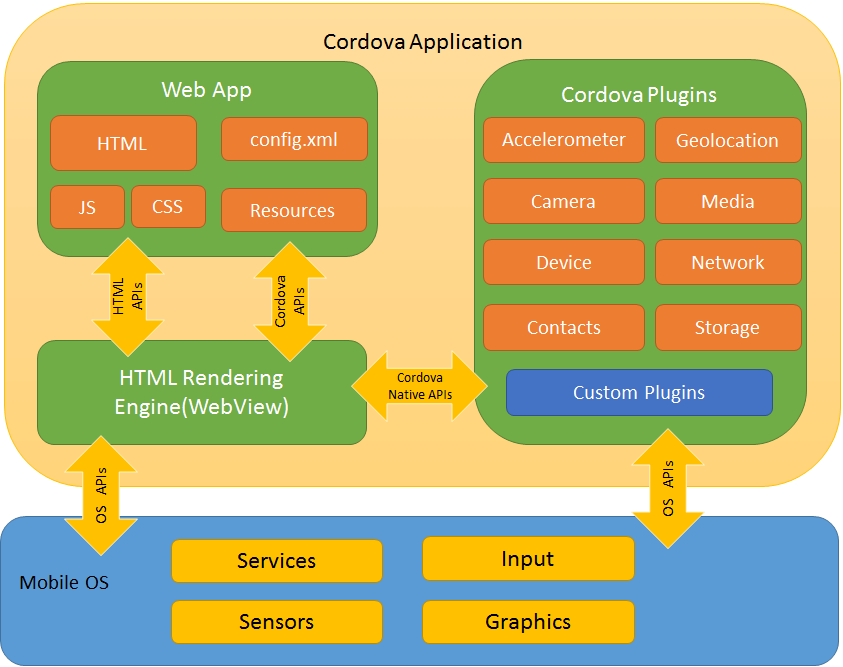
\includegraphics[width=0.2\textwidth]{./img/cordova_arquitectura.png}
      \caption{Vista principal de un acta.}
      \end{center}
    \end{figure}

      \subsubsection{Convocar xogadores}
      Nas accións habituais que debe realizar un árbitro, habitualmente o 
primeiro paso é cubrir no papel os nomes dos xogadores que se atopan presentes 
no encontro coas fichas identificativas de cada un de eles aporta.

      Como o obxectivo é eliminar o papel e simplificar o traballo do árbitro 
e da federación, a acta do encontro contén todos os xogadores que 
se atopan inscritos no equipo correspondente coa sua foto polo que xa non son 
precisas as fichas en papel de cada un de eles e o árbitro non ten que escribir 
os nomes dos integrantes dos equipos, se non que únicamente debe seleccionar 
cales se atopan no campo.

      Tamén ten a posibilidade de editar o dorsal do xogador para este encontro 
en concreto xa que en algunhas competicións é habitual que cambien de camiseta 
segundo o partido.

      Por último existe a opción de engadir un novo xogador de xeito 
manual, útil para o caso no que o árbitro teña que crear un acta manualmente ou 
para cando un novo xogador é engadido a un clube pero non é dado de alta na 
aplicación a tempo, e se o árbitro accede, este pode ser engadido a acta de 
xeito manual e competir sen problemas

    \begin{figure}[h!]
      \begin{center}
      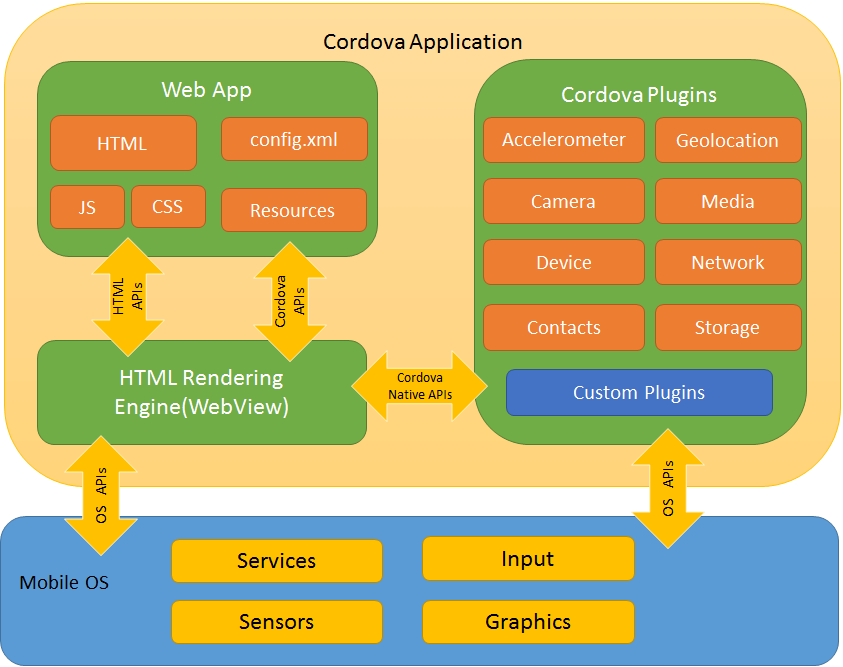
\includegraphics[width=0.2\textwidth]{./img/cordova_arquitectura.png}
      \caption{Seleccionar xogadores presentes no encontro.}
      \end{center}
    \end{figure}

      \subsubsection{Inicio e fin do partido}
      O seguinte paso a hora de xestionar a acta dun encontro é indicar cando 
comeza o mesmo, para isto disponse de un botón que só se mostra cando non 
comezou aínda o mesmo e que se encarga de introducir un evento de comezo.

      En este momento atoparase dispoñible o boton que permite arrancar e deter 
o \textbf{cronómetro} co fin de poder xestionar o encontro de xeito interactivo 
e que todos os eventos introducidos, leven incorporado o momento no que se 
produciron.

      Non é obrigatorio utilizar o cronómetro polo que os eventos poden ser 
engadidos en calquera momento e non se almacenará o minuto no que se produciron.

      Do mesmo xeito, pódese engadir un evento de fin de encontro nunha das 
opcións desplegables do menú superior dereito e que redirixirá ao árbitro a 
páxina de asinado de acta.

    \subsection{Finalización do encontro}
    Cando un árbitro decide rematar un encontro, accederá a esta última vista 
da aplicación onde poderá engadir un texto coa información de posibles 
\textbf{incidencias} que ocorreran durante o encontro e que deben ser postas en 
coñecemento da federación como algún tipo de agresión ou o motivo polo que un 
partido tivo que ser finalizado antes de tempo.

    \begin{figure}[h!]
      \begin{center}
      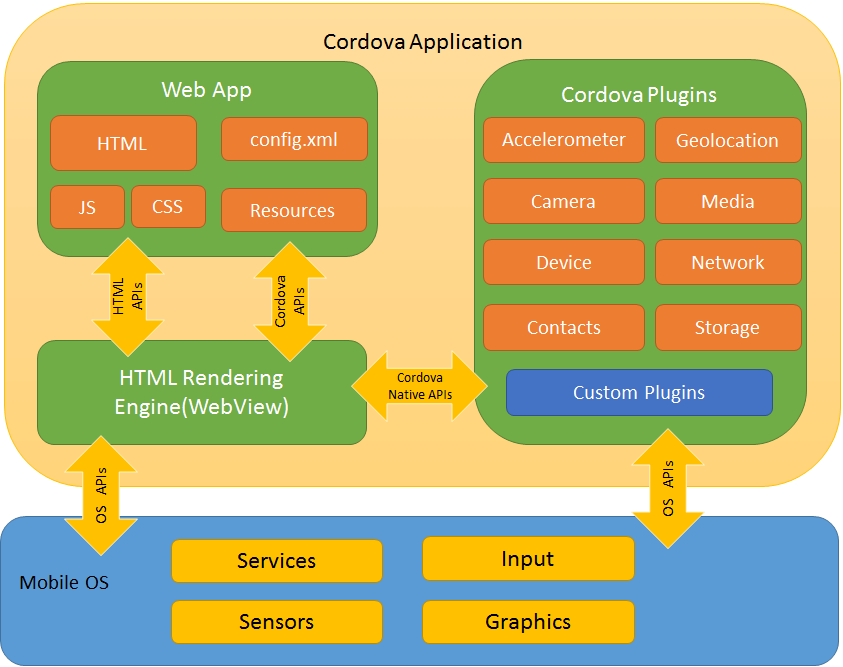
\includegraphics[width=0.2\textwidth]{./img/cordova_arquitectura.png}
      \caption{Fin de encontro.}
      \end{center}
    \end{figure}

    Dende o menú superior dereito pódese acceder directamente aos eventos que 
ocorreron durante o partido para mostrarlle as persoas que asinarán de cada 
equipo co fin de que poidan confirmar que realmente os eventos gardados na 
acta, son certos.

    A vista ten varias lapelas, unha para o árbitro e outra para cada un dos 
equipos onde poderán asinar a acta tantas persoas como sexa preciso.

    Unha vez se faga click no botón de asinar de algunha das lapelas, 
mostrarase unha listaxe coas persoas que poden asinar de cada equipo ou do 
equipo arbitral.

    Para realizar a sinatura, a persoa debe dispoñer de conta creada na base de 
datos da federación na que debeu de indicar un código PIN previamente que é o 
que permite asinar a acta.

    No caso de xogadores creados dende a propia aplicación móbil, poderase 
asinar a acta sen dispoñer de código PIN, deixando o oco baleiro.

    \begin{figure}[h!]
      \begin{center}
      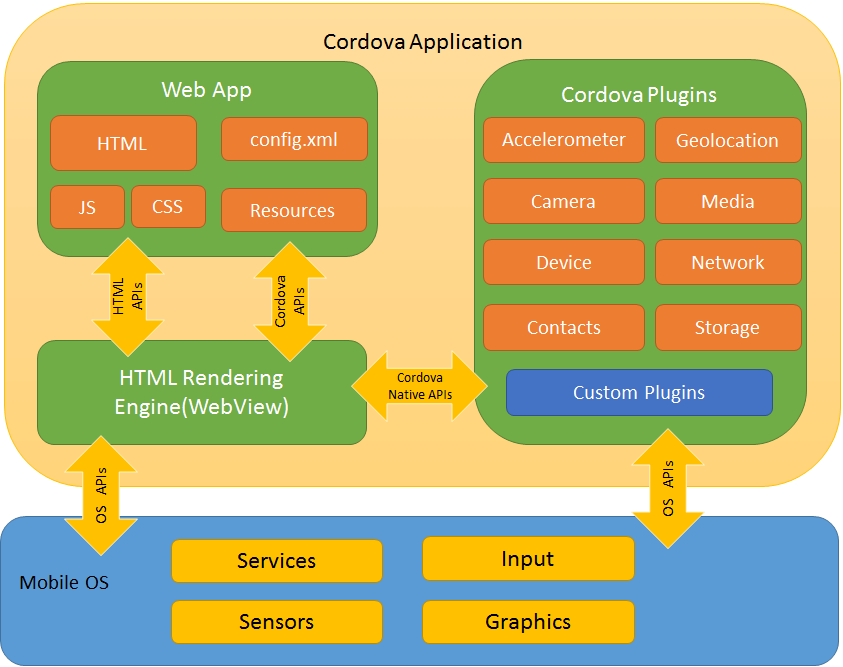
\includegraphics[width=0.2\textwidth]{./img/cordova_arquitectura.png}
      \caption{Sinatura de un acta.}
      \end{center}
    \end{figure}

  \section{Multideporte}
  Un dos obxectivos iniciais era conseguir que a aplicación puidera adaptarse 
de xeito moi sinxelo a novos deportes, inicialmente comezaríase co fútbol pero 
todo o deseño debía estar orientado cara este finalidade.

  \subsection{Deporte}
  Para iso creouse unha Store que contén a información do deporte que a 
aplicación está xestionando actualmente e que pode ser actualizado e cambiado 
por outro de xeito moi sinxelo.

  Por outro lado, cada deporte debe extender a unha clase xenérica Sport que 
define unha serie de métodos que todos os deportes deben implementar e que 
definen como se realizan certas accións sobre os datos en cada deporte.

  \begin{description}
   \item [Eventos] A lista de eventos que se poden realizar en ese deporte.
   \item [Evento por tipo] Que permite recuperar un obxecto Evento a partir da 
clave do seu tipo.
   \item [Icono por tipo] Que devolve o icono que identifica un Evento de un 
tipo para renderizalo en algunha parte da aplicación como a lista de eventos.
   \item [Campo primario] É unha función que calcula o resultado para 
almacenar no campo primario da acta en función da lista de eventos para ese 
encontro e de cada deporte. En fútbol devolve únicamente a suma de eventos de 
tipo gol.
   \item [Campo secundario] Similar ao campo anterior pero para introducir 
información no campo secundario da acta, no caso do fútbol, no campo secundario 
almacena as faltas do encontro e esta función devolve a suma de faltas que hay 
no partido.
  \end{description}

  Esta implementación fai que sexa tremendamente sinxelo engadir un novo 
deporte, básicamente sería crear unha nova clase que extendese os métodos 
correspondentes coa funcionalidade concreta de ese deporte.

  \subsection{Eventos}
  Do mesmo xeito, cada deporte ten os seus propios eventos polo que se definíu 
unha forma de engadir eventos de xeito sinxelo, co fin de que a incorporación 
de un novo deporte resultase o máis trivial posible.

  Actualmente podemos dividir os eventos en dóus tipos:

  \begin{description}
    \item [De control] Son eventos xenéricos de xestión como cambiar de parte, 
ou comezar un encontro que non é habitual que vaian a cambiar xa que son 
habitualmente os mesmos en todos os deportes.
    \item [De deporte] Son eventos concretos de cada deporte como engadir un gol 
ou unha tarxeta, a súa vez divídense en:
      \begin{description}
       \item [Evento] É un tipo de evento de deporte que únicamente permite ser 
engadido ou eliminado, non dispón de un comportamento especial.
       \item [Evento con causa] Ese tipo de evento engade tamén unha causa aos 
eventos xa que é habitual que se precise indicar o motivo polo que se producíu 
un evento como por exemplo cando o árbitro expulsa a un xogador con unha 
tarxeta vermella.
         \item [Evento de puntuación] Tipo de evento que permite actualizar os 
campos de resultados, primario e secundario de forma automática ao ser engadido.
      \end{description}

  \end{description}

  Existe un compoñente de React para incorporar os eventos de control dentro 
da vista que lista os eventos dun partido e que calquera evento de este tipo, 
definindo unha clase como a establecida para os eventos de control cos detalles 
do seu funcionamento, pode utilizar.
\todo{engadir imaxe de exemplo}

  Por outra banda temos tamén un compoñente de React para introducir os eventos 
deportivos na lista de eventos dun partido e cada evento novo debe crear un 
novo compoñente que defina a vista a mostrar cando se desexe engadir un evento 
de este tipo no encontro.

  En definitiva, para crear un novo evento débese definir unha clase Javascript 
coas propiedades do mesmo e que extenda ao SportEvent.

  Tamén é preciso engadir unha clase de React que defina a vista que se 
mostrará ao intentar engadir o evento durante o encontro (habitualmente unha 
ventá modal) e por último débese engadir o evento creado anteriormente, dentro 
da lista de eventos que ten ese deporte e que se atopan na clase que define as 
propiedades de dito deporte.

  \section{Deseño da DB}
  VACmatch Mobile estaba pensado inicialmente para integrarse co sistema de 
xestión de competicións que estamos a desenvolver con VACmatch Web que dispón 
dunha API de comunicacións que se atopa montada sobre unha base de datos 
relacional.

  É por iso que o modelo de datos estába pensado para unha base de 
datos relacional e tivo que ser adaptado para utilizar unha non relacional 
orientada a documentos.

  Prácticamente todas as entidades foron desnormalizadas para incluir 
información necesaria e en algún caso comprimironse dúas entidades en unha soa 
como é o caso de Call e Member que foron unidas dentro de Person como se indica 
no gráfico seguinte.

    \begin{figure}[h!]
      \begin{center}
      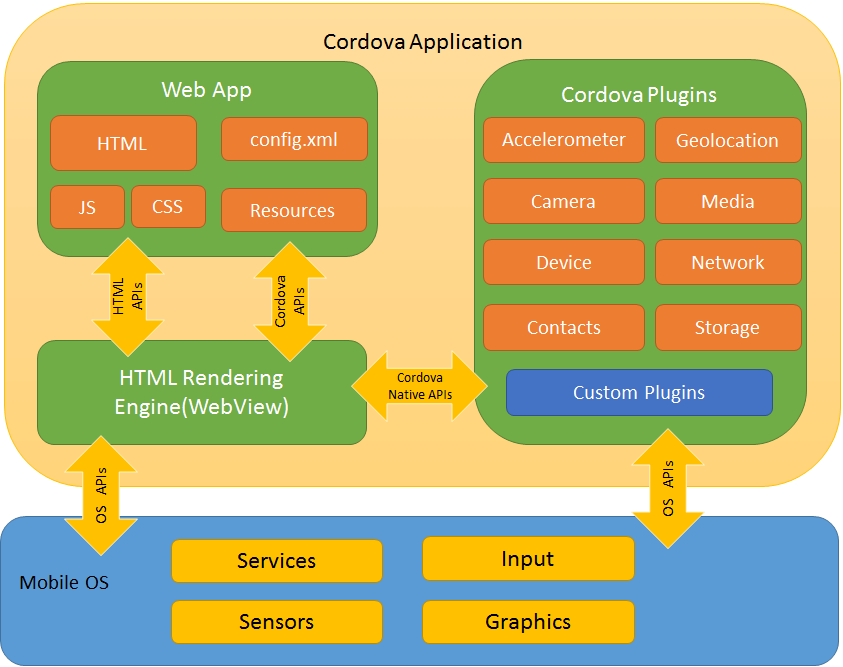
\includegraphics[width=0.2\textwidth]{./img/cordova_arquitectura.png}
      \caption{Esquema base de datos de Person.}
      \end{center}
    \end{figure}

  \section{I18n}
  Para a xestión da internacionalización da aplicación utilizouse a librería 
React Intl que provee unha serie de compoñentes de React e unha API sinxela 
para formatear datas, números e strings, incluindo pluralización e xestión de 
traduccións.

  Esta librería da a posibilidade de engadir un contexto aos textos que se 
internacionalizan o cal facilitará a labor do traductor que se encargue de 
engadir ou modificar un idioma, proveendo dunha información extra sobre o texto 
que debe traducir.

  Únicamente é preciso definir os compoñentes cos seus correspondentes 
atributos como se mostra no código seguinte e a propia ferramenta xenera 
ficheiros .json seguindo o esquema de carpetas e ficheiros da aplicación con 
toca a información recopilada.

     \begin{lstlisting}[frame=single, caption=Exemplo de internacionalización 
na label de un 
botón.]
        <RaisedButton label={
            <FormattedMessage
                id='report.show.events'
                description='Events button'
                defaultMessage='Events'/>
        } secondary={true} style={style.button}/>
    \end{lstlisting}

  Do mesmo xeito, a librería permite facer internacionalización de xeito 
programático sen utilizar compoñentes de react, a través de unha serie de 
funcións de javascript.

  Ademáis é preciso realizar as traduccións aos diferentes idiomas, cada un 
en un ficheiro de javascript diferente e con un formatado de pares cadea/valor.

  \section{Inxección de dependencias}
  Durante o realización do proxecto xurdíu problema entre os servizos xa que 
moitos precisan dos outros para realizar comprobacións de forma circular.

  A existencia destas dependencias circulares leva a que sexa imposible 
determinar a relación entre eles polo que é preciso deseñar un pequeno sistema 
de inxección de dependencias.

  A solución tomada é moi similiar a implementación que realiza Spring, 
dispoñemos dunha factoría que se encarga de crear un obxecto para cada servizo 
e a continuación inxéctanse uns dentro dos outros.

  Cada vez que se chama a factoría para recuperar un servizo, a factoría 
devolve o servizo coas súas dependencias inxectadas no seu interior polo que 
resolvemos o problema de xeito sinxelo.

  A continuación pódese ver un exemplo da factoría que se encarga de crear os 
servizos:

       \begin{lstlisting}[frame=single, caption=Exemplo de internacionalización 
na label de 
un botón.]

let ServiceFactory = {
  isInitialized: false,
  _servicesList: new Map(),

  constructor () {
    this._personService = new PersonService()
    this._reportService = new ReportService()
    this._refereeService = new RefereeService()
    // Without dependencies
    this._teamService = new TeamService()
    // Inject dependencies
    this._eventService.ReportService = this._reportService
    this._eventService.PersonService = this._personService
    this._eventService.TeamService = this._teamService
    ...
    // Add services to the exposed list
    this._servicesList.set('ReportService', this._reportService)
    this._servicesList.set('PersonService', this._personService)
    this._servicesList.set('TeamService', this._teamService)
    this.isInitialized = true
  },

  getService  (type) {
    if (!this.isInitialized) {
      this.constructor()
    }
    let service = this._servicesList.get(type)
    if (!service) {
      console.log('Error getting ', type, ' service')
    }
    return service
  }

}
    \end{lstlisting}

  Cómpre tamén comentar as dificultades que implica a inxección de dependencias 
ao realizar testing unitario xa que non se poden aproveitar as funcionalidades 
que aporta Jest, o framework de testing, que permiten automatizar a creación de 
mocks e obriga a crear manualmente os mocks dos servizos e inxectalos dentro do 
servicio a testear en cada test.

  \section{Testing e Integración continua}
  O testing é unha parte fundamental nun proxecto e concretamente nun proxecto 
de software libre no que a comunidade pode colaborar e onde poden 
participar persoas sen un coñecemento moi profundo da aplicación, polo que se 
fai totalmente imprescindible garantizar que calquera cambio non rompa a 
integridade da aplicación.

    \subsection{TDD e BDD}
  Neste proxecto seguironse diversas prácticas de Test Driven Development 
(TDD) e Behaviour Driven Development (BDD) comezando por unha definición das 
diversas tarefas do proxecto como tests de aceptación das funcionalidades e 
rematando pola realización de tests unitarios.

      \paragraph{Tests de aceptación} Estos tests son destinados a determinar 
se foron cumplidos os requisitos de unha certa funcionalidade, sempre 
centrándose na parte funcional e alonxándose dos detalles de implementación.

      Para isto utilízanse unha linguaxe simple de dominio para definir os 
requisitos funcionáis, en este proxecto baseamonos no seguinte:

        \begin{description}
         \item [Como ....] afectado ou realizador da funcionalidade.
         \item [Quero ...] acción a realizar.
         \item [Cando ...] momento ou caso no que debe realizarse.
        \end{description}

        Un exemplo de test de aceptación:

        \emph{Como árbitro quero que o resultado se actualice automáticamente 
ao engadir un novo gol}.

      \paragraph{Tests unitarios} Estos tests centranse en comprobar o 
funcionamento de xeito aislado dos diversos sistemas e centrándose en que cada 
proba sexa un caso totalmente independente do resto.

      En este proxecto crearonse tests unitarios centrados nos servizos da 
aplicación, que son os elementos máis importantes da mesma xa que son os que 
definen a lóxica de negocio.

      Para a realización de este tipo de tests é fundamental a utilización de 
mocks, obxectos que imitan o comportamento de obxectos reais de xeito 
controlado o cal permite simular o comportamento dos obxectos dependentes.
      Esto é fundamental para asegurar o illamento da funcionalidade e eliminar 
a dependencia de outros elementos a hora de realizar as probas unitarias.

    \subsection{Jest}
    É unha librería para realización de testing automático en aplicacións 
ReactJS que facilita.

    A continuación móstrase un test de exemplo do módulo de eventos no que se 
pode observar os compoñentes que o forman.

    Inicialmente defínese dentro da sección ''describe`` unha ''historia de 
usuario`` que contén a información xeral sobre o caso de uso, dentro da cal 
pódense realizar diversos tests, no exemplo que vemos, o caso de uso é ''Crear 
un evento deportivo''.

    Dentro do caso de uso vemos un bloque ``beforeEach'' que permite 
inicializar variables para cada novo test que se realice, eliminando de este 
xeito a dependencia entre os tests das variables que utilizan.

    Dentro do bloque ``describe'' defínense os diversos tests de esta historia 
de usuario dentro dos bloques ``it''.

    Ao realizar tests unitarios é habitual a utilización de obxectos mock que 
imitan a funcionalidade de outros.

    En Jest todos os obxectos son mocks e non é preciso definilos todos así, 
cambiando un pouco a forma de traballar habitualmente, aquí débese definir ao 
comezo do ficheiro aqueles que non van a ser mockeados a través da 
seguinte sentencia:

    \begin{lstlisting}[frame=single]
     jest.dontMock('../../src/app/models/report/status/StartedStatus')
    \end{lstlisting}

    Tamén é habitual querer darlle un comportamento por defecto aos mocks que 
se utilizan, por exemplo no seguinte trozo de código estamos facendo que cando 
se chame a función ``findById'' do obxecto ``reportService''  co un só 
parámetro, que o obxecto devolva un callback cos parámetros indicados, neste 
caso unha Acta por defecto (defaultReport) e un valor nulo como segundo 
parámetro.

    \begin{lstlisting}[frame=single]
  spyOn(reportService, 'findById').andCallFake(function (anyReportId, callback){
    callback(defaultReport, null)
  })
    \end{lstlisting}

    Unha vez definido o comportamento que queremos que teñan os mocks, debemos 
chamar ao método real do obxecto que estamos testeando e así teremos totalmente 
illado o comportamento do método a testear

    Finalmente utilizamos a cláusula ``expect'' para indicar resultados 
esperados, no caso de exemplo que mostramos a continuación, estamos a indicar 
que a chamada ao método findById de reportService foi realizada pero tamén é 
posible indicar valores que debe devolver, negacións ou outras validacións 
incluso máis complexas.

    \begin{lstlisting}[frame=single]
      expect(reportService.findById).toHaveBeenCalled()
    \end{lstlisting}

    A continuación mostramos o caso de test anterior completo a modo de exemplo.

    \begin{lstlisting}[frame=single, caption=Exemplo de test no módulo e eventos 
utilizando Jest.]
      describe('create Sport Event', function () {

        beforeEach(function () {
          defaultPerson = new Person(null, '', '', '', '', false, false, '', 
'',   '')
          defaultTeam = new Team(null, 'Team name')
          defaultReport = new Report(null, '', '', ReportStatus.READY, 
defaultTeam, defaultTeam, [])
          defaultEvent = new EventElements.Event('event', '1', defaultPerson, 
      defaultTeam, 'goal', 1, 'cause', 1)
          reportService = new ReportService(jasmine.createSpy('PersonService'), 
      jasmine.createSpy('TeamService'), jasmine.createSpy('EventService'), 
      jasmine.createSpy('SignService'))
          personService = new PersonService(jasmine.createSpy('ReportService'), 
      jasmine.createSpy('TeamService'), jasmine.createSpy('AuthService'))
          teamService = new TeamService()
          eventService = new EventService(reportService, personService, 
  teamService)
        })

        it('Create a new Sport Event with valid parameters', function () {

          spyOn(reportService, 'findById').andCallFake(function (anyReportId, 
      callback) {
            callback(defaultReport, null)
          })

          spyOn(personService, 
    'findByPersonIdReportIdAndTeamId').andCallFake(function   (anyPersonId, 
    anyReportId, anyTeamId, callback) {
            callback(defaultPerson, null)
          })

          spyOn(teamService, 'findById').andCallFake(function (anyTeamId, 
  callback)  {
            callback(defaultTeam, null)
          })

          spyOn(EventDao, 'create').andCallFake(function (reportId, person, 
team, eventType, matchTime, cause, timestamp, callback) {
            callback(defaultEvent, null)
          })

          eventService.create(defaultEvent.reportId, defaultEvent.person, 
      defaultEvent.team,
            defaultEvent.type, defaultEvent.matchTime, defaultEvent.text, 
      defaultEvent.timestamp,
            (event, err) => {
              expect(event).toEqual(defaultEvent)
              expect(event).not.toBe(null)
              expect(err).toBe(null)
          })

          expect(reportService.findById).toHaveBeenCalled()
          
expect(personService.findByPersonIdReportIdAndTeamId).toHaveBeenCalled()
          expect(teamService.findById).toHaveBeenCalled()
          expect(EventDao.create).toHaveBeenCalled()
        })
  \end{lstlisting}

    \subsection{Travis CI}
    A medida que a aplicación foi medrando, xurdíu a necesidade de simplificar 
traballos como a búsqueda de erros ou o mantemento da aplicación, buscando 
garantizar que se mantén a integridade da mesma en todo momento e non se 
introducen erros polo que se decidíu engadir tests unitarios na aplicación.

    Da mesma maneira lanzóuse unha primeira vesión estable do proxecto polo 
que tamén se decidíu engadir un sistema de integración continua ao mesmo co 
fin de garantizar que a aplicación xerada na rama de producción é funcional, 
compila en todo momento e pasa tódolos tests.

    Para isto utilizóuse Travis CI como sistema integración para o que se 
engadíu un ficheiro ``.travis.yml'' no que se lle indica a Travis diversos 
parámetros de configuración como as versións de Javascript coas que debe poñer 
a proba o funcionamento do programa, os scripts a executar para instalar 
dependencias e executar o programa, as ramas de desenvolvemento sobre as que 
debe actuar, no noso caso ``master'' e ``development`` ou as notificacións que 
debe enviar ao finalizar un traballo como por correo electrónico ou utilizando 
un servizo de mensaxería instantánea como Slack.

    Nesta integración xurdíu un problema derivado do sistema de construcción 
utilizado no proxecto, Gulp, que nos axuda a automatizar tarefas como a 
compilación, a execución dos tests ou o deploy da aplicación, e do framework de 
tests, Jest xa que a execución de este último a través de Gulp non devolvía os 
erros ao resolver os tests como resultado da función se non que o facía a 
través de un callback polo que foi preciso engadir na tarefa ''test`` definida 
en Gulp, o control de este caso para evitar falsos positivos na execución dende 
Travis.
